% Geometrie der Multipolentwicklung: Quellpunkt r', Aufpunkt r, Winkel gamma
% Gemeinsamer Stil für alle Abbildungen (TikZ -> SVG, siehe figures/build.mjs).
%
% Farben sind Platzhalter ("Sentinels"): build.mjs ersetzt sie im SVG durch
% CSS-Variablen, damit die Abbildungen im hellen und dunklen Modus passen.
% Andere Farben (auch schwarz/weiß) bricht der Build mit Fehler ab.
%
%   fg    Linien, Beschriftung          -> --dark
%   mu    Hilfslinien, Achsen, Maße      -> --gray
%   acc   das eine Konzept der Abbildung -> --secondary (Lime/Oliv)
%   blue  zweite Größe, negative Ladung  -> --fig-blue
%   warm  dritte Größe, positive Ladung  -> --fig-warm
%   bg    Seitenhintergrund (Aussparen)  -> --light
%
% Kein \clip verwenden: pdftocairo macht daraus Clip-Gruppen, in denen exakt
% waagerechte/senkrechte Linien verschwinden. Berechnete Kurven schneidet
% gen/*.py selbst am Rahmen ab.
\documentclass[tikz,border=3pt]{standalone}
\usepackage{amsmath,amssymb,bm}
% Text serifenlos wie die Seite, Mathe in Computer Modern wie KaTeX
\renewcommand{\familydefault}{\sfdefault}
\usetikzlibrary{arrows.meta,calc,decorations.markings,patterns,3d,positioning,angles,quotes}

\definecolor{fg}{RGB}{1,2,3}
\definecolor{mu}{RGB}{4,5,6}
\definecolor{acc}{RGB}{7,8,9}
\definecolor{blue}{RGB}{10,11,12}
\definecolor{warm}{RGB}{13,14,15}
\definecolor{bg}{RGB}{16,17,18}

% Vektoren wie auf der Website (KaTeX \mathbf)
\newcommand{\vv}[1]{\mathbf{#1}}

\tikzset{
  every picture/.style={fg, line width=0.8pt, line cap=round, line join=round,
    >={Stealth[length=5.5pt,width=4.4pt]}},
  every node/.style={font=\small},
  % Linientypen
  main/.style={line width=0.9pt},
  thin/.style={line width=0.5pt},
  aux/.style={mu, line width=0.5pt, dash pattern=on 2.5pt off 2pt},
  axis/.style={mu, line width=0.6pt, ->},
  vec/.style={line width=1.1pt, ->},
  field/.style={line width=0.7pt, postaction={decorate},
    decoration={markings, mark=at position #1 with {\arrow{Stealth[length=4.5pt,width=3.6pt]}}}},
  field/.default=0.5,
  % Flächen
  soft/.style={fill=#1, fill opacity=0.14},
  soft/.default=acc,
  % Ladungen
  qpos/.style={circle, fill=warm, inner sep=0pt, minimum size=9pt,
    path picture={\draw[bg, line width=0.9pt] ($(path picture bounding box.center)+(-2pt,0)$) -- +(4pt,0)
      ($(path picture bounding box.center)+(0,-2pt)$) -- +(0,4pt);}},
  qneg/.style={circle, fill=blue, inner sep=0pt, minimum size=9pt,
    path picture={\draw[bg, line width=0.9pt] ($(path picture bounding box.center)+(-2pt,0)$) -- +(4pt,0);}},
  dot/.style={circle, fill=fg, inner sep=0pt, minimum size=3pt},
  % Beschriftung mit Aussparung, damit Linien den Text nicht kreuzen
  lbl/.style={fill=bg, inner sep=1.5pt},
  % Icons: kräftigere Linien, keine Schrift
  icon/.style={line width=1.6pt, >={Stealth[length=6pt,width=5pt]}},
}

\begin{document}
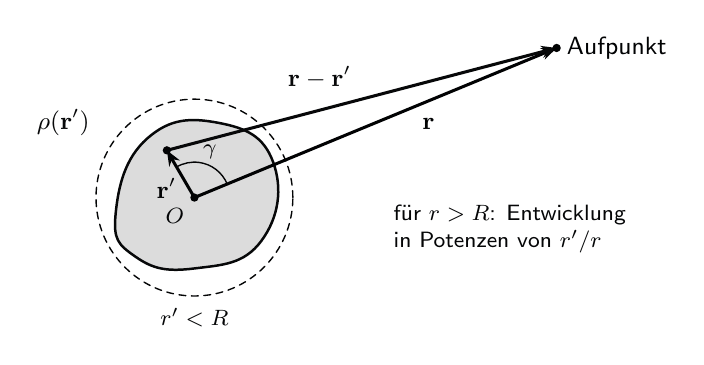
\begin{tikzpicture}
  \coordinate (O) at (0,0);
  % kompakte Ladungsverteilung
  \draw[acc, main, soft] plot[smooth cycle, tension=0.8] coordinates
    {(-1.0,-0.2) (-0.6,0.75) (0.3,0.95) (1.0,0.45) (0.85,-0.55) (0.0,-0.9) (-0.75,-0.75)};
  \node[acc, anchor=east] at (-1.2,0.95) {$\rho(\vv r')$};
  \draw[aux] (O) circle (1.25);
  \node[mu, font=\footnotesize, anchor=north] at (0,-1.28) {$r'<R$};
  \coordinate (Q) at (-0.35,0.6);
  \coordinate (P) at (4.6,1.9);
  \node[dot] at (O) {};
  \node[mu, font=\footnotesize, anchor=north east] at (O) {$O$};
  \draw[vec] (O) -- (Q) node[pos=0.5, anchor=north east, inner sep=1pt] {$\vv r'$};
  \draw[vec] (O) -- (P) node[pos=0.6, anchor=north west] {$\vv r$};
  \draw[vec, acc] (Q) -- (P) node[pos=0.5, anchor=south east] {$\vv r-\vv r'$};
  \node[dot] at (Q) {};
  \node[dot] at (P) {};
  \node[anchor=west] at (P) {Aufpunkt};
  \pic[draw, mu, thin, angle radius=0.45cm, "$\gamma$"{font=\footnotesize, text=mu}, angle eccentricity=1.35] {angle = P--O--Q};
  \node[mu, font=\footnotesize, align=left, anchor=west] at (2.4,-0.4) {für $r>R$: Entwicklung\\in Potenzen von $r'/r$};
\end{tikzpicture}
\end{document}
